\documentclass[12pt]{article}
\usepackage[margin=1in]{geometry} 
\usepackage{amsmath,amsthm,amssymb,amsfonts}
\usepackage{enumerate,listings,graphicx,epstopdf,siunitx}
\usepackage{color}
\graphicspath{~/Documents/school/fall16/stat586/hw3}

\sloppy
\definecolor{lightgray}{gray}{0.5}
 
\newcommand{\N}{\mathbb{N}}
\newcommand{\Z}{\mathbb{Z}}
\newcommand{\normD}[3]{\frac{1}{\sqrt{2\pi #1^2}}exp(\frac{-( #2 - #3)^2}{2 #1^2})} 
\newenvironment{problem}[2][Problem]{\begin{trivlist}
\item[\hskip \labelsep {\bfseries #1}\hskip \labelsep {\bfseries #2.}]
  \vspace{1 cm}
}{\end{trivlist}}

\begin{document}
\title{Homework Set 4}
\author{Taylor Bodin}
\maketitle

\section*{Problem 3.35} %TODO: Figures
\subsection*{a.} %TODO: fig_3_35_a
\begin{align*}
  f_{X|X>0} &= \frac{P(X \leq x, 0<X<\infty)}{P(0<X<\infty)} \\
  &= \begin{cases} 
        \frac{f_X(x)}{P(0<x)}, & 0 < x < \infty \\
        0, & otherwise 
     \end{cases} \\
  &= \begin{cases} 
        \frac{1}{2\sqrt{2\pi\sigma^2}}exp(\frac{-x^2}{2\sigma^2}), & 0 < x < \infty \\
        0, & otherwise 
      \end{cases}
\end{align*}

%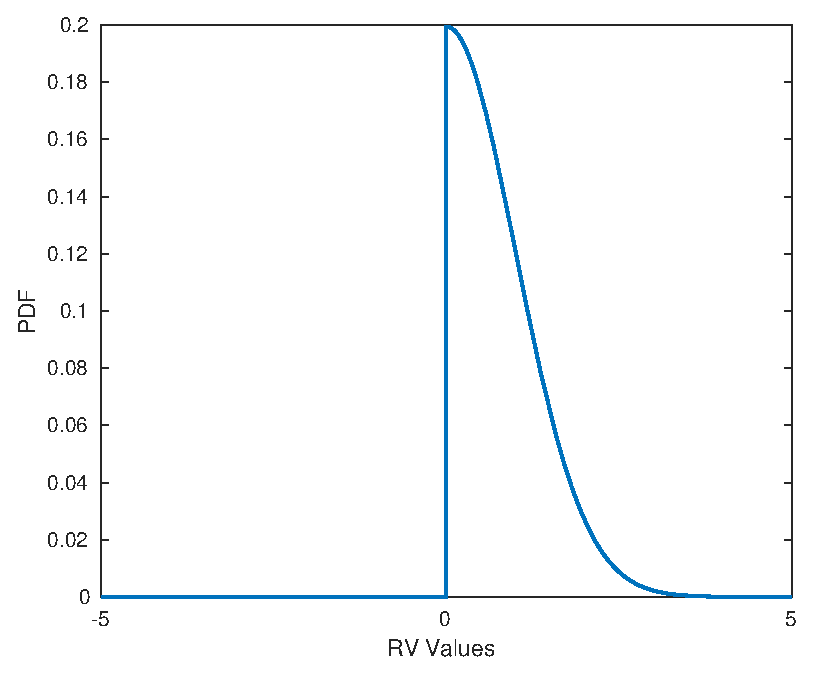
\includegraphics [width=4in]{fig_3_35_a.eps}
\subsection*{b.} %TODO: fig_3_35_b
\begin{align*}
  f_{X||X|>3} &= \frac{P(X \leq x, -3<X<3)}{P(-3<X<3)} \\
  &= \begin{cases} 
    \frac{f_X(x)}{P(-3<x<3)}, & -3 < x < 3 \\
    0, & otherwise 
  \end{cases} \\
  &= \begin{cases} 
    \frac{\frac{1}{2\sqrt{2\pi\sigma^2}}exp(\frac{-x^2}{2\sigma^2})}
    {Q(\frac{-3}{\sigma}) - Q(\frac{3}{\sigma})}, & 0 < x < \infty \\
    0, & otherwise 
  \end{cases} \\
  &= \begin{cases} 
    \frac{1}{2\sqrt{2\pi\sigma^2}}exp(\frac{-x^2}{2\sigma^2})
    \frac{1}{1 - 2Q(\frac{3}{\sigma})}, & 0 < x < \infty \\
    0, & otherwise 
  \end{cases}
\end{align*}

%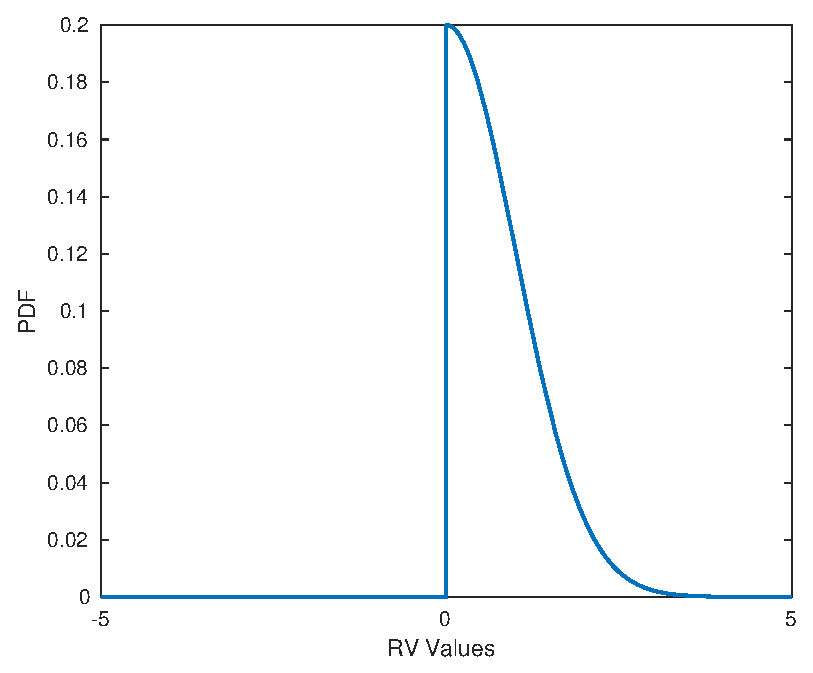
\includegraphics [width=4in]{fig_3_35_b.eps}
\subsection*{c.} %TODO: fig_3_35_c
\begin{align*}
  f_{X||X|<3} &= \frac{P(X \leq x, -3>X \cup  X>3)}{P(-3>X \cup  X>3)} \\
  &= \begin{cases} 
    \frac{f_X(x)}{P(-3>X \cup  X>3)}, &  -3>X \textrm{ or } X>3\\
    0, & otherwise 
  \end{cases} \\
  &= \begin{cases} 
    \frac{\frac{1}{2\sqrt{2\pi\sigma^2}}exp(\frac{-x^2}{2\sigma^2})}
    {1- Q(\frac{-3}{\sigma}) + Q(\frac{3}{\sigma})}, & -3>X \textrm{ or } X>3 \\
    0, & otherwise 
  \end{cases} \\
  &= \begin{cases} 
    \frac{1}{2\sqrt{2\pi\sigma^2}}exp(\frac{-x^2}{2\sigma^2})
    \frac{1}{2Q(\frac{3}{\sigma})}, &  -3>X \textrm{ or } X>3 \\
    0, & otherwise 
  \end{cases}
\end{align*}

%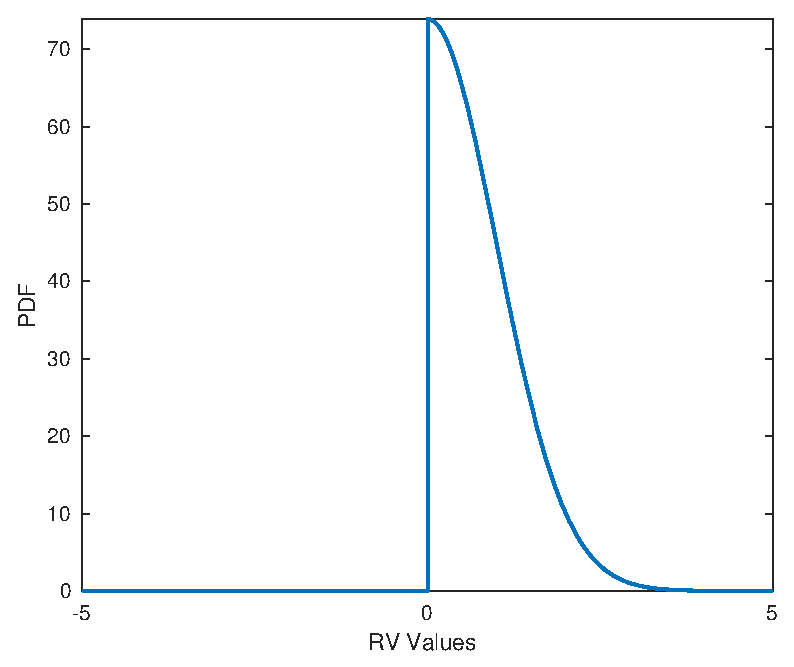
\includegraphics [width=4in]{fig_3_35_c.eps}

\section*{Problem 3.37}
\subsection*{a.}
\subsubsection*{Find an expresion for $P_{m=0|X=x}$}
\begin{align*}
  P_{m=0|X=x} &= \frac{f_{x|m=0}P(m=0)}{f_{x|m=0}P(m=0)+f_{x|m=1}P(m=1)} \\
  &= \frac{.5\normD{\sigma}{x}{0}}{.5\normD{\sigma}{x}{0}+.5\normD{\sigma}{x}{1}} \\
  &= \frac{exp(\frac{-x^2}{2\sigma^2})}
    {exp(\frac{-x^2}{2\sigma^2})+exp(\frac{-(x-1)^2}{2\sigma^2})} \\
  &= \frac{\sqrt{e}}{\sqrt{e}+e^x} 
\end{align*}
\subsubsection*{Find an expresion for $P_{m=1|X=x}$}
\begin{align*}
  P_{m=1|X=x} &= \frac{f_{x|m=1}P(m=1)}{f_{x|m=0}P(m=0)+f_{x|m=1}P(m=1)} \\
  &= \frac{.5\normD{\sigma}{x}{1}}{.5\normD{\sigma}{x}{0}+.5\normD{\sigma}{x}{1}} \\
  &= \frac{exp(\frac{-(x-1)^2}{2\sigma^2})}
    {exp(\frac{-x^2}{2\sigma^2})+exp(\frac{-(x-1)^2}{2\sigma^2})} \\
  &= \frac{e^x}{\sqrt{e}+e^x} 
\end{align*}
\subsubsection*{Find X such that $P \geq .9$ for each case and E otherwise}
\[
\begin{cases}
  1, & x > 2.697 \\
  E, & -1.698 < x < 2.697 \\
  0, & x < -1.697 
\end{cases}
\]
\subsection*{b.}
\begin{align*}
  P(E) &= P(X<2.697|m=1)P(m=1)+P(X>-1.697|m=0)P(m=0) \\
  &= (1 - Q(\frac{2.697-1}{1})).5 + Q(\frac{-1.697}{1}).5 \\
  &= .9552(.5) + .9552(.5) = .9552
\end{align*}
\subsection*{c.}
\begin{align*}
  P(\textrm{error}) &= P(X>2.697|m=0)P(m=0)+P(X<-1.697|m=1)P(m=1) \\
  &= Q(2.697)(.5) + 1 - Q(-2.697)(.5) \\
  &= Q(2.697) = .0035
\end{align*}

\section*{Problem 3.39}
\subsection*{a.}
\begin{align*}
  f_{V|V>1} &= \begin{cases} 
     \frac{f_V(v)}{P(1<v)}, & 1 < v < 2 \\
        0, & otherwise 
     \end{cases} \\
    &= \begin{cases} 
      \frac{.5}{.5}, & 1 < v < 2 \\
        0, & otherwise 
      \end{cases} \\
    &= \begin{cases} 
      \frac{1}{4}, & 1 < v < 2 \\
        0, & otherwise 
      \end{cases}
\end{align*}
\subsection*{b.}
\begin{align*}
  f_{V|} &= \begin{cases} 
    \frac{f_V(v)}{P(\frac{1}{2}<v<\frac{3}{2})}, & \frac{1}{2}<v<\frac{3}{2} \\
        0, & otherwise 
     \end{cases} \\
    &= \begin{cases} 
      \frac{.5}{.5}, & \frac{1}{2}<v<\frac{3}{2} \\
        0, & otherwise 
      \end{cases} \\
    &= \begin{cases} 
      \frac{1}{4}, & \frac{1}{2}<v<\frac{3}{2} \\
        0, & otherwise 
      \end{cases}
\end{align*}
\subsection*{c.}
\begin{align*}
  F_{V|\frac{1}{2}<V<\frac{3}{2}} &= 
  \begin{cases} 
    0, & V<\frac{1}{2} \\
    \frac{f_V(v) - f_V(.5)}{f_V(1.5) - f_V(.5)}, & \frac{1}{2}<v<\frac{3}{2} \\
    1, & V>\frac{3}{2}
  \end{cases} \\
 &= \begin{cases} 
    0, & V<\frac{1}{2} \\
    v-\frac{1}{2}, & \frac{1}{2}<v<\frac{3}{2} \\
    1, & V>\frac{3}{2}
  \end{cases}  
\end{align*}

\section*{Problem 3.41}
\subsection*{Setup}
$R_{1 unit} = \lambda_n = \frac{1}{100} \textrm{days}^{-1}$ \\
$R_{system} = \sum_{n=1}^{10} R_{1_unit} = (10)\frac{1}{100} = \frac{1}{10} \textrm{days}^{-1}$

\subsection*{a.}
\[
  P(L_{system} > 100) = exp(-(\frac{1}{10} \textrm{days}^{-1})(10 \textrm{days})) = e^{-1} = .3679
\]
\subsection*{b.}
\[
  P(L_{unit} > 100) = exp(-(\frac{1}{100} \textrm{days}^{-1})(10 \textrm{days})) = e^{-1} = .9048
\]
\section*{Problem 3.43}
\subsection*{c.}
$R_{1 unit} = \lambda_n = \frac{1}{100} \textrm{days}^{-1}$ \\
$R_{system} = \sum_{n=1}^{10} R_{1_unit} = (10)\frac{1}{100} = \frac{1}{10} \textrm{days}^{-1}$

\subsection*{a.}
\begin{align*}
  P(S|x=200) &= \frac{P(S|x=200)P(S)}{P(S|x=200)P(S)+P(L|x=200)P(L)} \\
  &= \frac{.75(\frac{1}{100}exp(\frac{-200}{100}))}{.75(\frac{1}{100}exp(\frac{-200}{100})
    .25(\frac{1}{1000}exp(\frac{-200}{1000})} \\
  &= .8322
\end{align*}

\subsection*{b.}
\begin{align*}
  P(L|x=200) &= \frac{P(L|x=200)P(L)}{P(S|x=200)P(S)+P(L|x=200)P(L)} \\
  &= \frac{.25(\frac{1}{1000}exp(\frac{-200}{1000}))}{.75(\frac{1}{100}exp(\frac{-200}{100})
    .25(\frac{1}{1000}exp(\frac{-200}{1000})} \\
  &= .1678
\end{align*}

\section*{Problem 3.45}
\subsection*{a.}
\begin{align*}
  SSE &= \sum_{n=1}^k \left( F_n - (1 - exp(\frac{-x_n^2}{2\sigma^2}))^2 \right) \\
  \frac{d}{d\sigma^2}SSE &= \frac{d}{d\sigma^2}\sum_{n=1}^k \left( F_n - (1 - exp(\frac{-x_n^2}{2\sigma^2}))^2 \right) \\
  0 &= \frac{2}{\sigma^3}\sum_{n=1}^k \left( F_n - (1 - exp(\frac{-x_n^2}{2\sigma^2}))\right)exp(\frac{-2x_n^2}{2\sigma^2})x_n^2
\end{align*}

\subsection*{b.}
\begin{align*}
  SSE &= \sum_{n=1}^k \left( log(1-Fn) + \frac{-x_n^2}{2\sigma^2} \right)^2 \\
  \frac{d}{d\sigma^2}SSE &= \frac{d}{d\sigma^2} \sum_{n=1}^k \left( log(1-Fn) + \frac{-x_n^2}{2\sigma^2} \right)^2 \\
  0 &= \sum_{n=1}^k 2(log(1-F_n) + \frac{x_n^2}{2\sigma^2}(\frac{-x_n^2}{2\sigma^4}) \\
  0 &= \sum_{n=1}^k 2(x_n^2 log(1-F_n) + \frac{x_n^4}{2\sigma^2}) \\
  \frac{1}{\sigma^2} \sum_{n=1}^k x_n^4 &= \sum_{n=1}^k x_n^2 log(1-F_n) \\
  \sigma^2 &= -\frac{\sum_{n=1}^k x_n^4}{\sum_{n=1}^k x_n^2 log(1-F_n)}
\end{align*}

\end{document}
